% Mobile ad-hoc network
% Author: Dr. Ludger Humbert
% Source: https://haspe.homeip.net/projekte/ddi/browser/tex/pgf2
\documentclass{standalone}

\usepackage{tikz}
\usepackage{pgf}

\usepackage{xxcolor}

\usetikzlibrary{arrows,shadows,petri}
%                              wg. tokens
\newlength{\imagewidth}
\newlength{\imagescale}

\listfiles

\begin{document}

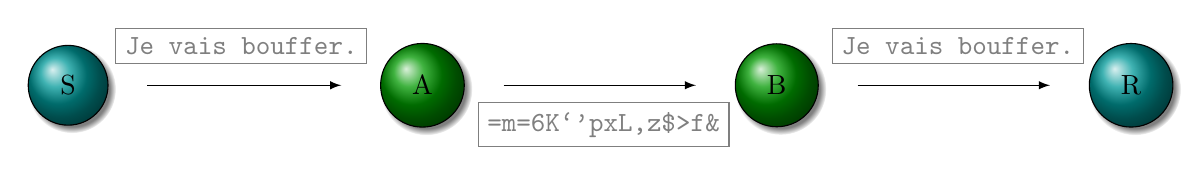
\begin{tikzpicture}[
    knoten/.style={
      shading=ball,
      circle,
      inner sep=.25cm,
      outer sep=.5cm,
      circular drop shadow,
      draw},
    /schriftstueck/.code 2 args={
      \fill[red!50, opacity=#2] #1 rectangle +(.6,.7);
      \foreach \y in {0pt,2pt,4pt,6pt,8pt,10pt,12pt,14pt}
       \draw [yshift=\y, opacity=#2] #1+(0.1,0.1) -- +(0.1,0.1);
      }
    ]

  \node at (0,.5) (knoten0) [knoten, ball color=cyan!60!black] {S};

  \node[rectangle,draw,opacity=.5] at (2.2,1)  (ack10) {\texttt{Je vais bouffer.}};

  \node at (4.5,.5) (knoten1) [knoten, ball color=green!60!black] {A};

  \node[rectangle,draw,opacity=.5] at (6.8,0)  (ack11)  {\texttt{=m=6K`'pxL,z\$>f\&}};

  \node at (9,.5) (knoten2) [knoten, ball color=green!60!black] {B};

  \node[rectangle,draw,opacity=.5] at (11.3,1)  (ack10) {\texttt{Je vais bouffer.}};


  \node at (13.5,.5) (knoten3) [knoten, ball color=cyan!60!black] {R};
  

  \path  [-latex] (knoten0) edge [] (knoten1);
  \path  [-latex] (knoten1) edge [] (knoten2);
  \path  [-latex] (knoten2) edge [] (knoten3);

\end{tikzpicture}

\end{document}
